% This is a template for doing homework assignments in LaTeX
\documentclass[twocolumn]{article} % This command is used to set the type of document you are working on such as an article, book, or presenation
\usepackage{geometry} % This package allows the editing of the page layout
\usepackage{amsmath}  % This package allows the use of a large range of mathematical formula, commands, and symbols
\usepackage{graphicx}  % This package allows the importing of images
\usepackage{mathtools}
\usepackage{enumitem}
\usepackage{outlines}
\usepackage{array}
\usepackage{graphicx}
\usepackage{amssymb}
\usepackage{multirow}
\usepackage{placeins}
\usepackage{relsize}
\usepackage{amsmath, amsthm, amssymb, amsfonts}

\graphicspath{{../images/}}

\DeclarePairedDelimiterX{\set}[1]{\{}{\}}{\setargs{#1}}
\NewDocumentCommand{\setargs}{>{\SplitArgument{1}{;}}m}
{\setargsaux#1}
\NewDocumentCommand{\setargsaux}{mm}
{\IfNoValueTF{#2}{#1} {#1\nonscript\:\delimsize\vert\allowbreak\nonscript\:\mathopen{}#2}}%
\def\Set{\set*}%
\newcommand{\problem}[2][]{\clearpage\begin{flushleft}
        \textbf{Problem #1}: \textit{#2} 
\end{flushleft}}
\newcommand{\sol}{\textbf{Solution}:} %Use if you want a boldface solution line
\newcommand{\maketitletwo}[2][]{\begin{center}
        \Large{\textbf{Homework 4}

        } % Name of course here
        \vspace{5pt}
        
        \normalsize{  % Your name here
        
        \today}        % Change to due date if preferred
        \vspace{15pt}
\end{center}}
\begin{document}

\tableofcontents


\section{Introduction}

\subsection{Qualities of Fungi}
The most significant characteristics of fungi that determine their decomposition rates are their moisture tolerance levels, hyphal extension rates, and competitiveness. 
\subsection{Relationship Between Moisture Tolerance and Competitiveness}
Fungi can have varying levels of moisture tolerance. However, their competitiveness—the ability to obtain more resources than other fungi—is inversely proportional to their moisture tolerance. Thus, fungi that thrive in humid climates, such as those that grow in tropical rainforests, will likely die off if they are in a dry climate where fungi with a weaker moisture tolerance grow.

\section{Fungi Characteristics}

\subsection{Fungi Interactions}
In order to accurately predict the rate at which fungi decompose different substrates, it is critical to understand how fungi interact with each other. If there are multiple species of fungi present in the same place, a single species or group of species may grow significantly faster than the rest. If this occurs, the competitive fungi will take up the limited resources that are stored in the substrate. Moreover, some fungi are also able to inhibit the speed that other fungi grow. 

\subsubsection{Competitiveness}
The competitiveness of species of fungi is represented by the variable, “c”, in the model. The competitiveness variable expresses a species’ ability to 

\subsection{Fungistasis}

Some fungi are capable of doing more than absorbing nutrients at a fast rate. There are species of fungi, such as Trichoderma, that can put some species of fungi into fungistasis, a condition that prevents affected fungi from decomposing substrates. Thus, fungi that inflict this state onto other fungi are infinitely more “competitive” than susceptible fungi as susceptible fungi completely stop growing. This is accounted for in the model by turning the competitiveness factor into 0. By doing this, the decomposition rate of affected fungi becomes negligible.

\subsection{Fungi Decomposition}

Fungi decomposition varies from the type of fungi doing the composing. Fungi that are competitive and have a higher hyphal extension rate decompose wood faster than fungi that are stress-tolerant and slow-growing. 

The substrate that a fungus decomposes significantly affects the fungus’ decomposition rate. For instance, if a fungus grows on wood, the amount of lignin in the wood can prevent it from decomposing woody fibers at a fast rate, and thus decreasing the growth rate as well. This is incorporated into our model through the “h” variable. Furthermore, the carbon-nitrogen ratio in both the substrate and growing fungi affect the rate at which carbon and nitrogen are consumed. If the carbon-nitrogen ratio in the substrate is not the same as the carbon-nitrogen ratio in the fungi that grow in the substrate, then the fungi will absorb more carbon or nitrogen molecules to make the ratios the same between fungi and the substrate.


\section{Environmental Effects on Fungi}

\subsection{Temperature}

\subsection{Humidity}

Consider the Köppen climate classification. This is a system for classifying different environments based on moisture, humidity and temperature. Incidentally, those are the three main environmental parameters that are important for fungal growth rates. For this model, we decided to combine all of three of these parameters into a single parameter(h). (h) represents how severe a given environment is given its Koppen climate classification.

\subsection{Light}
The amount of light a population of fungi is exposed to can have varying effects on the population’s growth. While most fungi grow faster in dark environments, some fungi, like Trichoderma spp., require light in order to sporulate. For a fungus like this, light increases the growth rate because the number of fungi rises and thus the rate of the population’s total growth rate becomes larger.

\subsection{Fungi Decomposition}

\subsection{Biodiversity and Varying Environments}

The number of unique species of fungi will make the total fungi population more resistant to changes in the environment. Biodiversity allows populations to possess a larger range of ideal environmental conditions. Consequently, when qualities of the environment change, groups of different types of fungi will be able to endure such shifts because different species thrive in different environments. Varying environmental conditions also give more species the opportunity to outcompete one another. Thus, one can expect for population numbers to remain consistent if a diverse group of fungi live in an environment that is constantly changing.

\section{Hyphal Extension and Wood Decomposition}
The relationship between hyphal extension and wood decomposition are directly proportional. If hyphal extension is intrinsically high then wood decomposition occurs fast as well. Some species of fungus that are slow growing and stress tolerant of their environment have lower rate of wood decomposition subsequently a lower hyphal extension rate therefore some species will not be able to consume as much wood mass. 

\section{Moisture Niche Width}

The moisture niche width refers to the range of values that a fungi is capable of growing in, while the moisture tolerance refers to how tolerant a given fungus is as environmental variables begin to shift away from its ideal growing condition. For the sake of this paper, we have decided to split the moisture niche into two variables, moisture tolerance ($m$) and ideal growing conditions ($h$).


\section{Model Discussion}

\noindent Our model uses the following parameters to represent the traits described above.

\section*{Environment}
$ D: $ Woody Decomposition Rate\\
$ K: $ Carrying Capacity\\
$ \beta : $  Effect of environment on growth\\ 
$ H: $ Environmental severity\\
$ N(t): $ Total population \\
$ S(t): $ Population of Sapotrophic Fungi\\
$ j:  $ Number of fungal species

\section*{Fungus}
$ r_i: $ Hyphal Extension Rate\\
$ h_i: $ Ideal severity\\
$ n_i(t): $ Population\\
$ m_i: $ Moisture tolerance \\
$ s_i: $ Sapotrophic/not sapotrophic\\ 
$ c_i: $ Competitiveness


\begin{equation} \label{Population}
    N(t) = \mathlarger{\mathlarger{\sum}}_{i=0}^{j} n_i
\end{equation}

\noindent Equation \ref{Population} defines our total population as a simple sum of each individual fungal population.

\begin{equation} \label{Sapotrophic}
    S(t) = \mathlarger{\mathlarger{\sum}}_{i=0}^{j} 
    \begin{cases}
	    0 & s_i = 0\\
	    r_i (n_i) & s_i = 1
    \end{cases}
\end{equation}

\noindent Equation \ref{Sapotrophic} defines our woody decomposition rate. For every sapotrophic fungi, the woody decomposition rate cretaes directly increases by the product of that fungi's growth rate and current population.

\begin{equation}\label{Growth rate}
    \frac{dn_i}{dt} = r_i \left(c_i - \beta\frac{\left| h_i - H\right|}{m_i} - \frac{N}{K} \right)
\end{equation}

Equation \ref{Growth rate} shows how we have chosen to simulate fungal performance. Note that a single fungus under ideal conditions would grow to the carrying capacity ($ K $ ) at ti's growth rate ($ r_i $ ). If the fungus were outside of it's ideal environment, then this would be indiciated in a difference between $ h_i $ and $ H $, which would lower the growth rate as well as the maximum capacity that the fungus could reach. This effect would be mitigated by a fungus having a higher moisture tolerance ($ m_i $ ). A similar effect occurs based on the ($ c_i $ ) of the fungus, which represents how well the fungus competes with other fungi in it's environment. A lower $ c_i $ would result in slower growth rate and a lower capacity for the fungus. This effect would be amplified as there is more biomass of competing fungi in the environment. 


\section{Model Analysis}
\subsection{Arid Conditions}
\noindent We first decided to run our model with three competing fungi. These fungi included two sapotrophic fungi and one non-sapotrophic fungal species. Of the sapotrophic fungi, one was a generalist fungi, while the other was a specalist adapted to semi-arid conditions. The non-sapotrophic species was a highly compettitive species adapted to more humid coniditons. Of the three of these fungi. In figure \ref{fig:f1}, we placed all three of these fungi into an arid environment to see how they would compete. The blue line represents fungus 1, the sapotrophic generalist. The yellow line represents fungus 2, the sapotrophic specialist. Finally, the green line represents our compettitive non-sapotrophic fungus. In \ref{fig:f1}, fungus 2 dies off quite quicklym but fungus 1 sustains until it is eventually overtaken by fungus 3. The outcome of this can be seen in \ref{fig:d1}, with a strong initial decomposition rate eventually falling off as fungus 3 becomes dominant.
\begin{figure}[bt]
	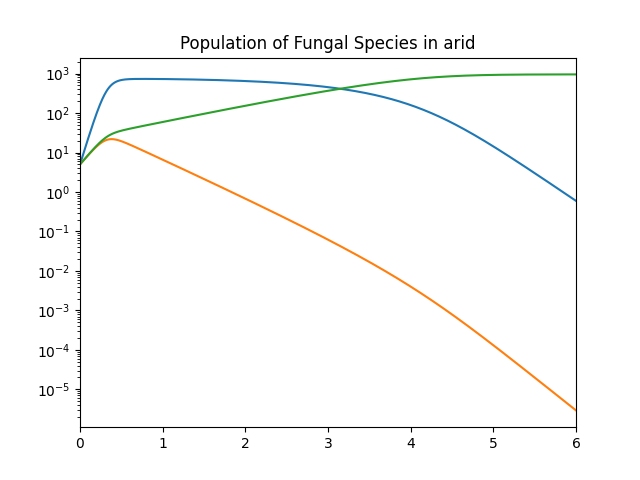
\includegraphics[width=\columnwidth]{figures/Figure_1.png}
      \caption{Fungal Growth in arid conditions, measured in tons of biomass}
      \label{fig:f1}
\end{figure}


\begin{figure}[bt]
	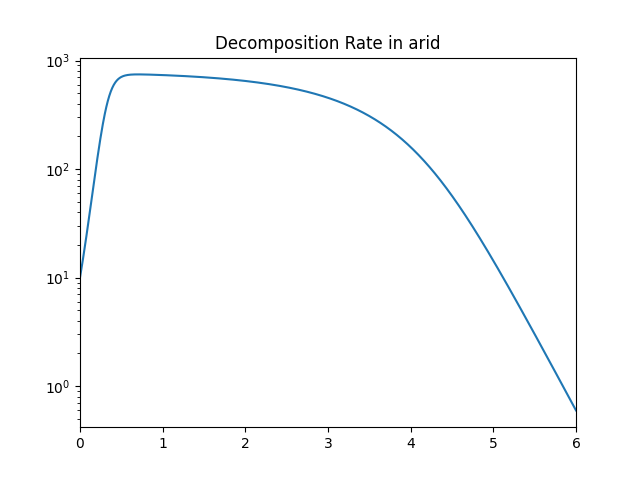
\includegraphics[width=\columnwidth]{figures/Figure_2.png}
      \caption{Woody Decomposition rate in arid conditions, measured in tons of biomass per year}
      \label{fig:d1}
\end{figure}

\subsection{Semi-Arid conditions}
\noindent Next, we decided to see how these same three fungi would perform in semi-arid conditions. In figures \ref{fig:f2} and \ref{fig:d2}, we set our $ H $ variable to a more hospitable environment to see how our different fungi would compete. As you can see in figure \ref{fig:f2}, the fungi interacted in a similar way to figure \ref{fig:d2}. This is because our non-sapotrophic fungi was simply too compettitive. As you can see in figure \ref{fig:d2}, our decompoisiton rate responded similarly to our previous model as well. 

\begin{figure}[t]
	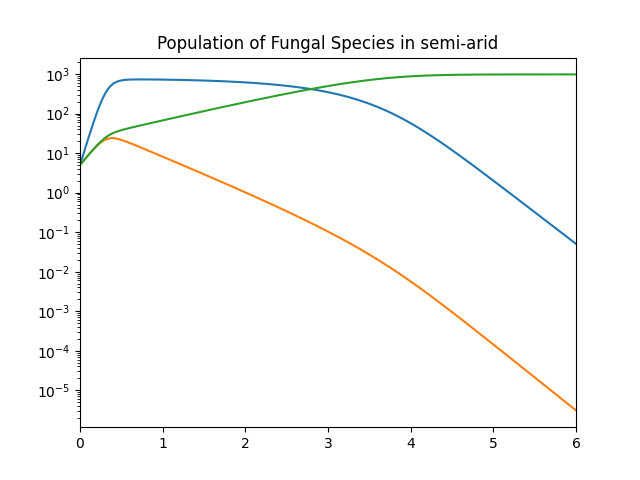
\includegraphics[width=\columnwidth]{figures/Figure_1_s.png}
      \caption{Fungal Growth in semi-arid conditions, measured in tons of biomass}
      \label{fig:f2}
\end{figure}
\begin{figure}[t]
	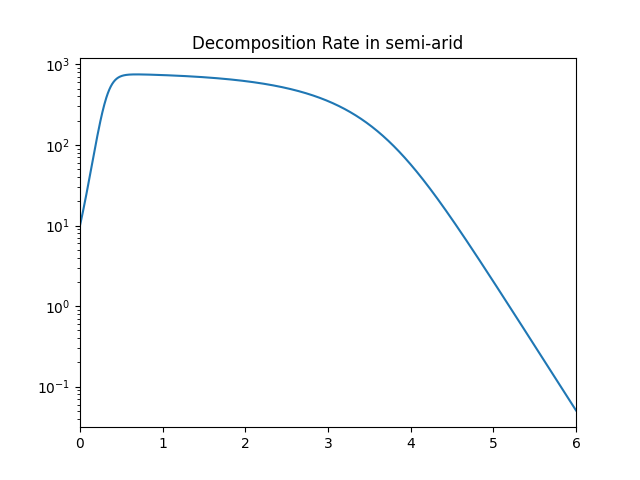
\includegraphics[width=\columnwidth]{figures/Figure_2_s.png}
      \caption{Woody Decomposition rate in semi-arid conditions, measured in tons of biomass per year}
      \label{fig:d2}
\end{figure}

\newpage
\section{Assumptions}

The model makes a few assumptions about the environment in which fungi grow. For all of the fungi analyzed by the model, the model assumes that resources, such as carbon and nitrogen, are constantly replenished as they are being absorbed. In addition, the amount of resources never rises either. Thus, significant changes in the amount of resources in the substrate are not accounted for.

Furthermore, the model does not explore how fungi may behave in the presence of other organisms. Bacteria, for example, may compete for the same resources as fungi and thus limit the amount of resources that fungi may absorb. In addition, other organisms, such as humans, may affect a fungus colony’s ability to grow. While the model accepts numerous parameters to make predictions regarding fungi growth and decomposition, these predictions are generalizations and are not necessarily accurate throughout an environment. For instance, there may be organisms around fungi that temporarily and/or permanently alter parts of the environment in which fungi grow, such as animals creating shelters that may prevent fungi from being reached by sunlight. 

\newpage
\section{Conclusion}

We conluded that fungal compettition is far more influencial on woody decomposition rate than the environment itself. Although fungi do react to the severity of their environmental condiitons, a highly comettive fungus will quickly kill off sapotrophic fungi in a region, resulting in a long-term decline of decomposition rate.

\bibliographystyle{plain}
\bibstyle{plain}
\bibliography{final_refs}

\bibdata{final_refs}

\end{document}

    
